\documentclass[11pt,a4paper]{article}
\usepackage[utf8]{inputenc}
\usepackage[english]{babel}
\usepackage{graphicx}
\usepackage{amsmath}
\usepackage{lmodern}
\usepackage[
	margin		= 22mm,
	top 		= 24mm,
	bottom 		= 10mm, 
	footnotesep = 2\baselineskip	
]{geometry}			
\usepackage{placeins}								% adds \FloatBarrier
\usepackage{float}									% adds [H] position argument aka 'the sledgehammer'
\usepackage{subcaption}								% adds subfigure
\usepackage{pdflscape}								% landscape pages
\usepackage{commath}								% adds vertical bar for \abs


%%%%%%%%%%%%%%%%%%%%%%%%%%%%%%%%%%%%%%%%%%%%%%%%%%%%%%%%%%%%%%%%%%%%%%%%%%%%%%%%%%%%%%%%%%%%%%%%%%%%%%%%%%%%%%%%%%%%%%%%%%%%%%%%%%%%%%%%%%%%%%%%%%%%%%%%%%%%%%%%%%%%%%%%%%%%%%%%%%%%%%%%%%%%%%%%%%%%%%%%

\usepackage{fancyhdr}
\pagestyle{fancy}
\fancyhf{}																	% clears all headers and footers
\fancyhead[c]{}
\fancyhead[l]{Aaron Schade}
\fancyhead[r]{\thepage}
\renewcommand{\headrulewidth}{1pt}
%\renewcommand{\footrulewidth}{1pt}

%\setlength{\headsep}{5mm}


%%%%%%%%%%%%%%%%%%%%%%%%%%%%%%%%%%%%%%%%%%%%%%%%%%%%%%%%%%%%%%%%%%%%%%%%%%%%%%%%%%%%%%%%%%%%%%%%%%%%%%%%%%%%%%%%%%%%%%%%%%%%%%%%%%%%%%%%%%%%%%%%%%%%%%%%%%%%%%%%%%%%%%%%%%%%%%%%%%%%%%%%%%%%%%%%%%%%%%%%
% formatting TOC
\usepackage{tocloft}

% distance to left margin, then distance from numbers to text
%\cftsetindents{section}{0em}{2em}
\cftsetindents{subsubsection}{23mm}{12mm}


%%%%%%%%%%%%%%%%%%%%%%%%%%%%%%%%%%%%%%%%%%%%%%%%%%%%%%%%%%%%%%%%%%%%%%%%%%%%%%%%%%%%%%%%%%%%%%%%%%%%%%%%%%%%%%%%%%%%%%%%%%%%%%%%%%%%%%%%%%%%%%%%%%%%%%%%%%%%%%%%%%%%%%%%%%%%%%%%%%%%%%%%%%%%%%%%%%%%%%%%


\usepackage[
	notes,
%	short,										% even first mention is shortened
	genallnames,								% when using \gentextcite for possessive cases, use all authors names
%	strict,										% erases the line before footnotes?
	urlnotes		= false,					% disable url, doi, eprint in notes but not in bibliography; alternatively: includeall  false OR doi % false, isbn % false, url % false,	eprint % false
	eprint			= false,
	backend 		= biber,					% biber's more advanced than bibtex
	autolang 		= other,
%	bibencoding 	= utf8,						% before: latin1 -> fucked up everything, couldnt recognise utf8 characters (duh!)
	compresspages]								% something like 321--328 in your .bib file would become 321–28
{biblatex-chicago}
\addbibresource{thesis.bib}

\AtEveryCitekey{\clearfield{isbn}}				% show isbn in bib, as before, but clear in citations
\AtEveryCitekey{\clearfield{issn}}	
\AtEveryCitekey{\clearfield{note}}	


\AtEveryCitekey{\clearfield{series}}	
\AtEveryCitekey{\clearlist{publisher}}	
\AtEveryCitekey{\clearlist{location}}	
\AtEveryCitekey{\clearfield{journaltitle}}	
\AtEveryCitekey{\clearfield{volume}}	
\AtEveryCitekey{\clearfield{pages}}	
\AtEveryCitekey{\clearfield{edition}}	
\AtEveryCitekey{\clearfield{date}}	
\AtEveryCitekey{\clearfield{year}}	
\AtEveryCitekey{\clearfield{institution}}	
\AtEveryCitekey{\clearfield{number}}	
\AtEveryCitekey{\clearfield{booktitle}}	
%\AtEveryCitekey{\clearname{editor}}	


\renewcommand*{\bibfont}{\small}
\DeclareDelimFormat{finalnamedelim}{\addspace\bibstring{and}\space}			% remove oxford comma



\usepackage[multiple, hang, bottom]{footmisc}
\setlength{\footnotemargin}{3mm}



%\usepackage{fnpct}											% improves kerning (spacing) of footnotemakrs above punctuation, could potentially do 'multiple' but doesnt work for citations (or at least its annoying with footnote citations)



%%%%%%%%%%%%%%%%%%%%%%%%%%%%%%%%%%%%%%%%%%%%%%%%%%%%%%%%%%%%%%%%%%%%%%%%%%%%%%%%%%%%%%%%%%%%%%%%%%%%%%%%%%%%%%%%%%%%%%%%%%%%%%%%%%%%%%%%%%%%%%%%%%%%%%%%%%%%%%%%%%%%%%%%%%%%%%%%%%%%%%%%%%%%%%%%%%%%%%%%



% important to load AFTER packages affecting referencing of any kind
\usepackage[
	linktoc			= all,								
	hyperfootnotes	= false, 				% footnotemarks are hyper to footnotetext - easily broken :/
%	hyperindex,								% numbers in index are hyper
	hidelinks, 								% just disables colour and border
%	bookmarksopen 	= false					% doesnt work to hide bookmarks, instead:
	pdfpagemode		= UseNone, 
	pdftitle 		= 'glorious title'
]{hyperref}




%%%%%%%%% misc %%%%%%%%%%%%%%%%%%%%%%%%%%%%%%%%%%%%%%%%%%%%%%%%%%%%%%%%%%%%%%%%%%%%%%%%%%%%%%%%%%%%%%%%%%%%%%%%%%%%%%%%%%%%%%%%%%%%%%%%%%%%%%%%%%%%%%%%%%%%%%%%%%%%%%%%%%%%%%%%%%%%%%%%%%%%%%%%%%%%%%%%%

%\usepackage{lipsum}


\usepackage{enumitem}
	\setlist{nosep}
%\usepackage{setspace}
%\usepackage{sectsty}
%\allsectionsfont{\centering}


%\usepackage{multicol}
%\newcommand{\fixspacing}{\vspace{0pt plus 1filll}\mbox{}}		% makes paragraphs not stretch in multicol - maybe?

\newcommand{\graph}{\medskip\noindent}
\newcommand{\osc}{\texttt{Oscillator}~}
\newcommand{\oscpop}{\texttt{OscPopulation}~}

\newcommand{\runK}{\code{runK()}~}
\newcommand{\runT}{\code{runT()}~}

\newcommand{\code}[1]{\texttt{#1}}

% makes underscore work in math mode? no? and we dont even want that -> just use \_ (its a special character)
%\catcode`_=12
%\begingroup\lccode`~=`_\lowercase{\endgroup\let~\sb}
%\mathcode`_="8000

\newcommand{\para}[1]{\paragraph{#1}\mbox{}\\}


%%%%%%%%%%%%%%%%%%%%%%%%%%%%%%%%%%%%%%%%%%%%%%%%%%%%%%%%%%%%%%%%%%%%%%%%%%%%%%%%%%%%%%%%%%%%%%%%%%%%%%%%%%%%%%%%%%%%%%%%%%%%%%%%%%%%%%%%%%%%%%%%%%%%%%%%%%%%%%%%%%%%%%%%%%%%%%%%%%%%%%%%%%%%%%%%%%%%%%%%
%%%%%%%%%%%%%%%%%%%%%%%%%%%%%%%%%%%%%%%%%%% to do %%%%%%%%%%%%%%%%%%%%%%%%%%%%%%%%%%%%%%%%%%%%%%%%%%%%%%%%%%%%%%%%%%%%%%%%%%%%%%%%%%%%%%%%%%%%%%%%%%%%%%%%%%%%%%%%%%%%%%%%%%%%%%%%%%%%%%%%%%%%%%%%%%%%%%
















%%%%%%%%%%%%%%%%%%%%%%%%%%%%%%%%%%%%%%%%%%%%%%%%%%%%%%%%%%%%%%%%%%%%%%%%%%%%%%%%%%%%%%%%%%%%%%%%%%%%%%%%%%%%%%%%%%%%%%%%%%%%%%%%%%%%%%%%%%%%%%%%%%%%%%%%%%%%%%%%%%%%%%%%%%%%%%%%%%%%%%%%%%%%%%%%%%%%%%%%
%%%%%%%%%%%%%%%%%%%%%%%%%%%%%%%%%%%%%%%%%%%%%%%%%%%%%%%%%%%%%%%%%%%%%%%%%%%%%%%%%%%%%%%%%%%%%%%%%%%%%%%%%%%%%%%%%%%%%%%%%%%%%%%%%%%%%%%%%%%%%%%%%%%%%%%%%%%%%%%%%%%%%%%%%%%%%%%%%%%%%%%%%%%%%%%%%%%%%%%%


\title{\vspace{30mm}\huge \bfseries A Study of Kuramoto Oscillators}
\author{Aaron Schade}




\begin{document}

\pagenumbering{gobble}


\maketitle
\vfill
\tableofcontents
\vfill


%%%%%%%%%%%%%%%%%%%%%%%%%%%%%%%%%%%%%%%%%%%%%%%%%%%%%%%%%%%%%%%%%%%%%%%%%%%%%%%%%%%%%%%%%%%%%%%%%%%%%%%%%%%%%%%%%%%%%%%%%%%%%%%%%%%%%%%%%%%%%%%%%%%%%%%%%%%%%%%%%%%%%%%%%%%%%%%%%%%%%%%%%%%%%%%%%%%%%%%%
\clearpage\pagenumbering{arabic}
\section{Theoretical study}















%%%%%%%%%%%%%%%%%%%%%%%%%%%%%%%%%%%%%%%%%%%%%%%%%%%%%%%%%%%%%%%%%%%%%%%%%%%%%%%%%%%%%%%%%%%%%%%%%%%%%%%%%%%%%%%%%%%%%%%%%%%%%%%%%%%%%%%%%%%%%%%%%%%%%%%%%%%%%%%%%%%%%%%%%%%%%%%%%%%%%%%%%%%%%%%%%%%%%%%%
\section{Numerical study}

\addcontentsline{toc}{subsection}{\\\textbf{Omegas normally distributed}}
{\Large\textbf{Omegas normally distributed}}
\subsection{$r_{\infty}(K)$ -- simulated vs predicted}


\subsubsection{Euler method}
%%%%%%%%%%%%%%%%%%%%%%%%%%%%%%%%%%%%%%%%%%%%%%%%%%%%%%%%%%%%%%%%%%%%%%%%
\para{Design and initiation}
My implementation of the Euler method is object-oriented. 
This may not be the computationally most efficient way, but I'm still somewhat coding beginner, so I appreciate the clarity that object-oriented programming affords.
The first type of object is simply an \osc with three fields: $\omega, \theta_{s-1}$ and $\theta_s$. 
In the Euler method it is enough to store the present and the last value of the state variable ($\theta$).
In the rest of this documentation, I will refer to \textit{simulation} time steps with the variable $s$ to differentiate it from the \textit{equation} time step $t$.

An \osc gets initiated with its natural frequency and the current-period $\theta_s$. 
The last-period $\theta_{s-1}$ is initiated as zero, since the first part of making an 'Euler step' forwards in time is handing over $\theta_{s}$ to $\theta_{s-1}$. 

The other object type is a population of oscillators, \code{OscPopulation}. 
It consists of a list of \code{Oscillators} and a construction mode, namely the probability distribution of the $\omega$.
When an \oscpop is initiated, for each \osc a natural frequency and initial phase are drawn from the respective types of random distribution. 
An \osc object is then initiated with those values for $\omega$ and $\theta_s$ and assigned to a place in the list within the \oscpop object.
The \oscpop object thus possess an indexable list of all oscillators.







%%%%%%%%%%%%%%%%%%%%%%%%%%%%%%%%%%%%%%%%%%%%%%%%%%%%%%%%%%%%%%%%%%%%%%%%
\para{Running the simulation}
The simulation has two functions, to run in two modes, \code{OscPopulation.runK()}~and \linebreak \code{OscPopulation.runT()}. 
I will get into the latter in subsection \ref{r(t)}.

To start a simulation for finding $r_\infty(K)$, a new \oscpop object gets created, passing the desired distribution type of $\omega$ to it.
Then \runK is run on this object.
It loops through the different values for K, starting with resetting the oscillators in the population, then Euler-stepping all oscillators through time until T and finally calculating $r_\infty(K)$. 
Take each in turn. 




\graph
The oscillators are reset by by finding new random values for $\omega$ and $\theta_s$ for all \code{Oscillators} and setting their field value equal to the newly calculated value. 
Same as during the original initiation, $\theta_{s-1}$ is set to zero.



\graph
The Euler-step function \code{OscPopulation.\_oneStepForAll()} is straight-forward in principle, but needs to be optimised for reasonable computation times. 
Originally, running task 1 with $ N = 100$, $K = [0, 4]$ and $dK = 0.1$ took about 45 minutes. 
Since the computation time likely increases exponentially with $N$ (more neighbouring oscillators have to be considered at \textit{each} step) the full compute time for $N=1000$ would have been unreasonable. 
Thus, I make use of the \code{numba} package which offers 'decorators' for functions. 
Decorators are functions which take functions as inputs and return modified functions.
In this case, the \code{@jit} decorator converts my Euler-step computation function into optimised machine code using the LLVM compiler. 
This can yield computation speeds similar to C or FORTRAN.\footnote{http://numba.pydata.org/}
It reduced the compute time for task 1 (with $N = 100$) from 45 minutes down to 4 minutes. 
%
To make it work, however, the function needs to take \code{nympy.ndarrays} as inputs, not objects, like originally the case in my object-oriented code. 
Therefore, I wrote the wrapper function \code{oneStepForAll} around \code{\_oneStepForAll} (which actually does the computation). 
It retrieves the values from the \oscpop object (a getter), puts them into temporary variables and then calls the optimised function \code{\_oneStepForAll} using those temporary variables (namely, arrays for $\omega, \theta_{s-1}, \theta_{s}$).
Finally, a setter writes the returned arrays for $\theta_{s-1}, \theta_{s}$ onto the \osc objects in the \oscpop. 

The core \code{\_oneStepForAll} function implements a standard Euler approximation.
First, the $\theta$ are stepped through time by handing the value of $\theta_{s}$ over to $\theta_{s-1}$.
In the next step, the sum of the the $sin$ of the differences between the last-period $\theta$ of oscillator $n$ ($\theta_{s-1}^n$) and all other oscillators $j$ ($\theta_{s-1}^j$) is computed:
\begin{align*}
	sum 					& = \sum_{j = 0}^N = \sin(\theta^j_{s-1} - \theta^n_{s-1}) \\
\intertext{From this, we can calculate the discrete $\Delta\theta_s^n$}
	\Delta\theta_s^n 		& = \omega_n + \frac{K}{N} *  sum \\
\intertext{The new $\theta_s$ of oscillator n is then}
	\theta^n_s 				& = \theta^n_{s-1} + \delta t \cdot \Delta\theta_s^n \\
\end{align*}
This is done for all N oscillators. 




\graph
After all oscillators have been stepped one simulation step $\delta s$ forward, this is repeated $\frac{T}{\delta t}$ times to get to the final time point $T$.
At this point, the limiting coherence parameter $r_(T)$ is calculated for the current $K$ and appended to a list of all $r_\infty(K)$. 

A new loop with the next $K$ begins until all $K$ values have been exhausted. 
The full results are returned as a list which is then graphed.
A scatter plot of $r_\infty(K)$, as opposed to a continuous line, has been chosen since a straight connection between points cannot be assumed.





\subsubsection{Program profile}
To make the structure of the code more clear and see which parts of the Euler-based simulation take the longest to compute, I profiled my python code. 
This profile shows which functions called which others as well as information about the execution of the respective function. 
After the name of the function, the first line shows the total time spent in this function (in itself and its children), the second how much time was spent only in itself and the third how many times the function was called.

\graph
The profile of the code for tasks 1 and 2 can be seen in figure \ref{profile12}.
Even when optimised, the computation time for these tasks is still 1h 30min. 
As the profile shows, almost all of this time (87\%) is spent in the main computation method \code{\_oneStepForAll}, which was called almost half a million times. 
The wrapper method retrieved 1.3bn and set over 800m values.


\begin{figure}[p]
	\centering
	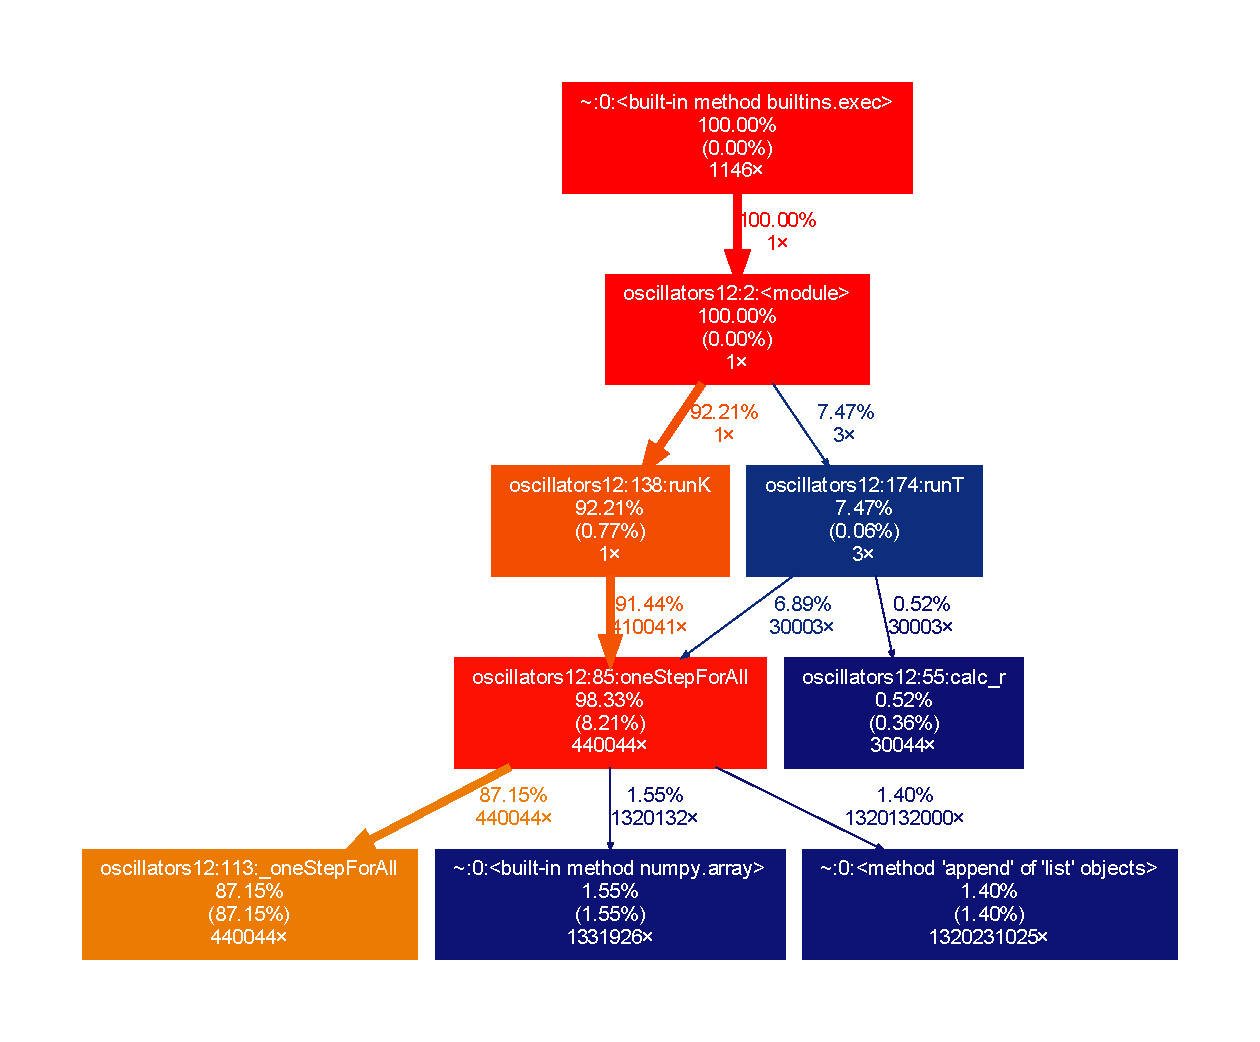
\includegraphics[width=\textwidth]{graphics/profile12.pdf}
	\caption{Profile of code for task 1 and 2}
	\label{profile12}
\end{figure}





\subsubsection{Numerical integration}
The strategy to integrate the consistency equation is to loop through different values of $r$ and check which ones make the right-hand side approximately equal to one. 
The precision of this approximation can be adjusted by changing the \code{rHysteresis} variable, which sets the acceptable range of values around 1 for the right-hand side of the consistency equation.
This is the \code{calc\_r\_integ(K)} function which takes $K$ as an input.

We now cycle through the different values for $K$ in a separate loop to get the values of the desired $r(K)$ relationship.
Since this is not a computationally-intensive step, I increased the resolution of $K$ to $\delta K = 0.01$. 
The hysteresis around the left-hand side value is $0.01$ and the step size of candidate $r$ is $\delta r = 0.001$.
The results are then graphed in figure \ref{1} together with the simulated points.




\subsubsection{Results}

\begin{figure}[H]
	\centering
	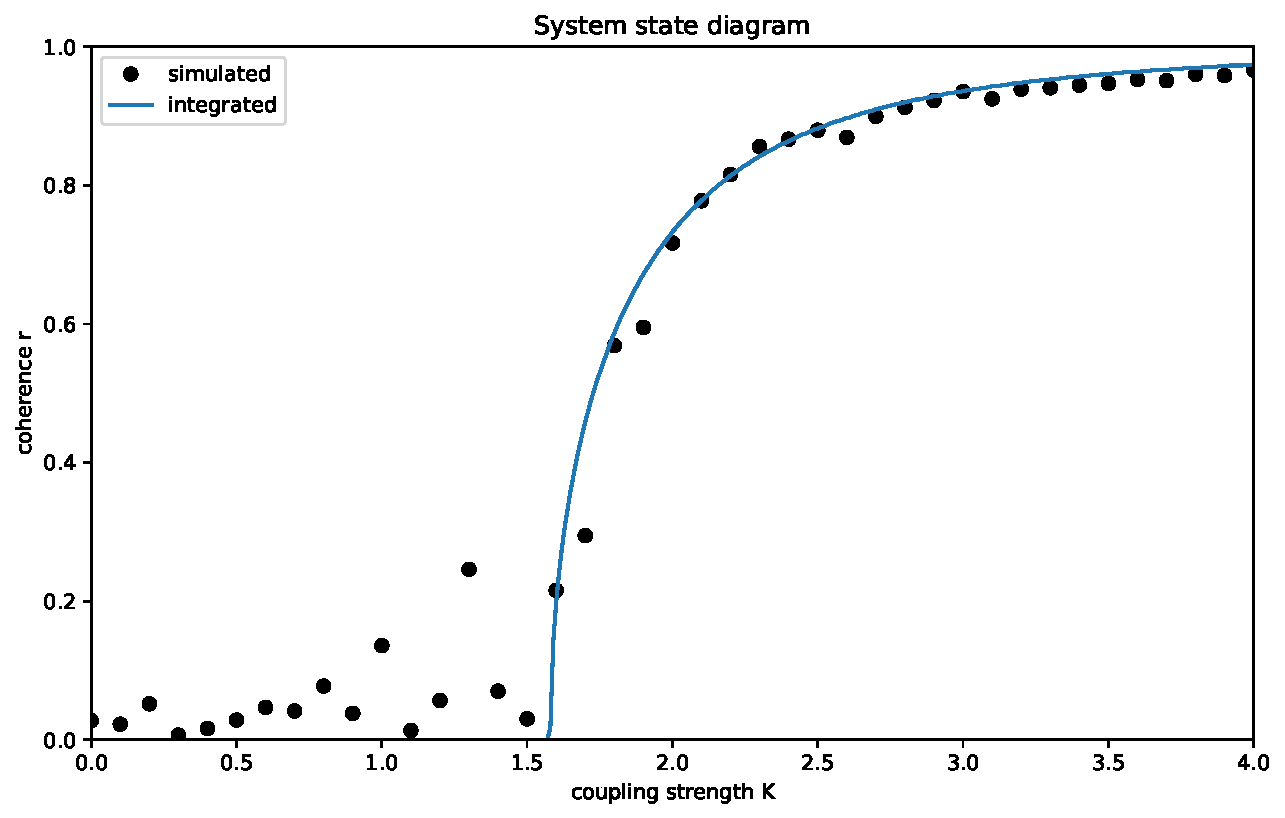
\includegraphics[width=0.9\textwidth]{graphics/1_K-vs-r_omegaDistr=normal_N=1000_1611577031.pdf}
	\caption{Diagram of limiting $r_\infty$ for different values of K}
	\label{1}
\end{figure}


The first observation is that, on the whole, the simulation values track the theoretical values quite closely. 
More precisely, the fit is \textit{very good} for $2<K$, \textit{good} in $0<K<1$ but has large deviations in $1<K<2$. 

My first impulse for improving the fit of the simulation lies in shrinking $\delta t$ to reduce the local and global error (which are proportional to $(\delta t)^2$ and $\delta t$, respectively).
Such errors happen because ODEs \textit{on paper} are continuous and essentially have infinite precision, which is impossible to achieve \textit{in silico}. 
In some non-linear dynamical models, such deviations in the discretised simulation can lead to \textit{qualitatively} different outcomes, especially when the system exhibits sensitive depends on initial conditions (ICs).
I do not believe the global error is large enough to cause the large positive deviations we observe just before the critical value $K_{crit} = 1.5958$. 

Instead, I hypothesise that the high-coherence observations in the range $1<K<1.5$ (which theory predicts should be very close to 0), are due to special sets of ICs. 
Out of all possible ICs of individual oscillators, a small subset will favour convergence of all oscillators to a (partially) synchronised state. 
If enough oscillators have correlated ICs, this could lead to higher-than expected coherence in the system.
If it is true that the outliers in the range $1<K<1.5$ are caused by unlikely constellations of ICs, then increasing N should diminish the occurrence of unlikely starting conditions. 
The probability of any IC to be coherence-favouring does not increase with N; in fact it may decrease because the union of coherence-favouring ICs between all oscillators shrinks.
As N gets larger, it thus becomes progressively less likely that a sufficiently large portion of the oscillator population (a 'critical mass') is randomly drawn with collectively-coherence-favouring ICs.
% eitiher focus on probability of individual oscillators IC to be favouring, or the collectivel ICs probability to be favouring







%%%%%%%%%%%%%%%%%%%%%%%%%%%%%%%%%%%%%%%%%%%%%%%%%%%%%%%%%%%%%%%%%%%%%%%%%%%%%%%%%%%%%%%%%%%%%%%%%%%%%%%%%%%%%%%%%%%%%%%%%%%%%%%%%
\clearpage
\subsection{$r(t)$ for $K = [1, 2,3]$} \label{r(t)}

The simulation procedure for is the same as for \runK, with 2 exceptions:
\begin{enumerate}
	\item there is still a $K$-loop (with limited values $K = [1,2,3]$), but there is no resetting of the population to new random values at the beginning of each such loop.
	\item $r(t)$ is now calculated at every (simulation!) time step $t$.
\end{enumerate}
The previous method of assigning new random values to the state variables of all oscillators did not work here for some reason. 
Instead, a bug occurred in which the final values of the last run were used as the starting values of a new run.%
	\footnote{.. despite many attempts to fix this bug. My hypothesis is that this is about memory management in python. Sometimes during other assignment of variables or objects, it merely creates a pointer instead of copying the value into a separate location in memory.}
Therefore I had to go another way: the \oscpop object is created anew in every loop. 
After the object is initiated with the right distribution of $\omega$, \runT is executed. 
It loops through all simulation time steps $s$. 
In one such loop, all oscillators are updated, then \code{calc\_r()} is called to compute $r_s$.

\code{calc\_r()} calculates $r_s$ in one of two different but equivalent ways. 
In one way, actual complex numbers are added up and divided by N. 
To get a value for $r$, the modulus of the resulting complex number is taken. 
$$ r_s = \frac{1}{N}       \cdot       \abs{\sum_{n=0}^N e^{ i \theta^n_s}}$$
The other way is to compute the double sum of real and imaginary component of the complex number (using the $sin$ and $cos$ relationships after DeMoivre and Euler).
These two sums are also divided by N, yielding the average real and imaginary component of the \oscpop at simulation time $s$. 
\begin{align*}
	realsum 	&= \sum_{n=0}^N \frac{\cos(\theta^n_s)}{N} \\
	imsum 		&= \sum_{n=0}^N \frac{\sin(\theta^n_s)}{N} \\
\intertext{From there, $r$ can be calculated through a square root:}
	r_s			&= \sqrt{realsum^2 \cdot imsum^2}
\end{align*}
I tried both versions to double check the results and to see whether one would give a performance boost over the other, but both have approximately the same speed.
In the end, \code{calc\_r()} returns a list of $r(t)$ which will be appended to a list-of-lists with the $r$ values for all chosen $K$. 
These different trajectories are once again graphed: figure \ref{2}.





\subsubsection{Results}

\begin{figure}[H]
	\centering
	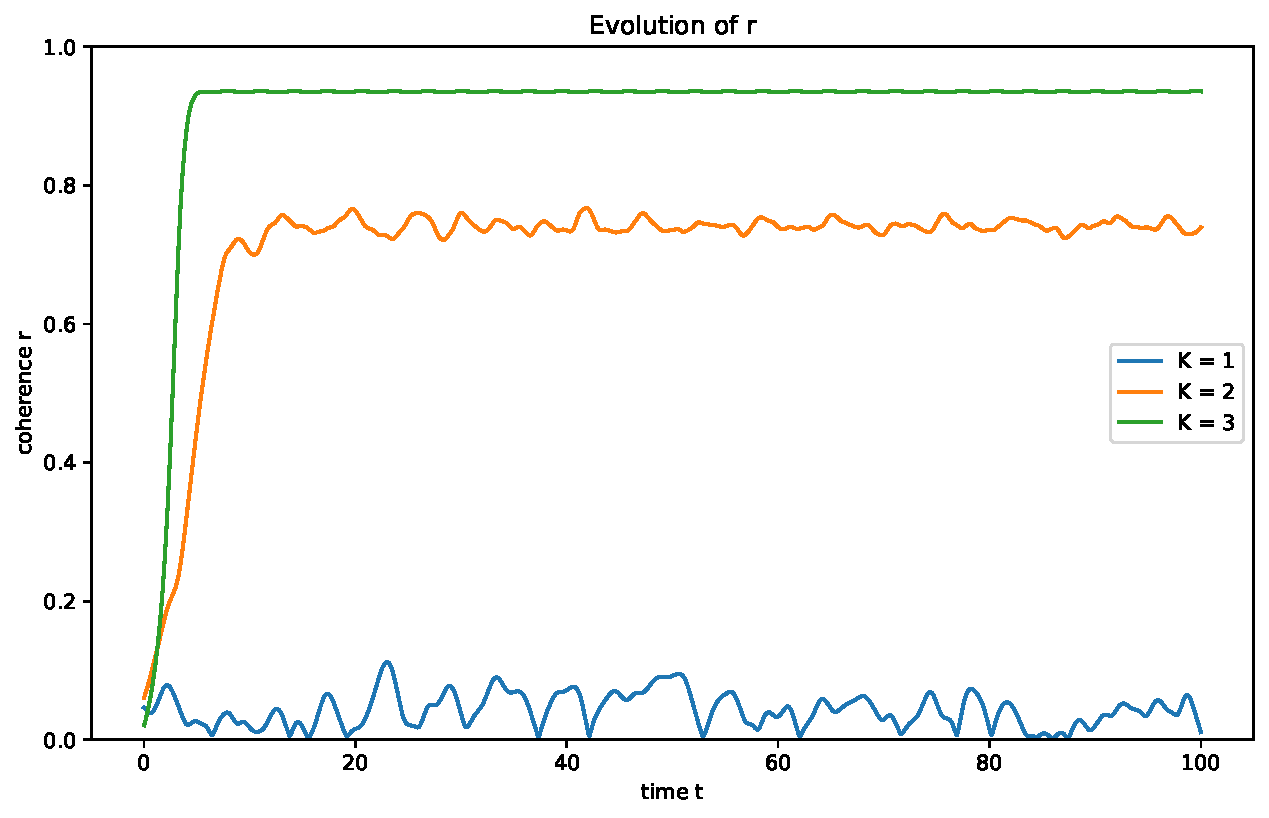
\includegraphics[width=0.9\textwidth]{graphics/2_t-vs-r_omegaDistr=normal_N=1000_1611577412.pdf}
	\caption{$r(t)$ over time for 3 different values of $K$}
	\label{2}
\end{figure}


Of note is firstly that populations with $K<K_{crit} \approx 1.5985$ do not converge to coherence, while those with $K>K_{crit}$ do. 
In this first sense, it is in agreement with theory. 
%
The second noticeable feature is that when convergence happens, it happens quickly, before $t = 10$.
% 
Thirdly, the consistency equation predicts essentially three ranges of $K$ with distinguishable features, as we can see in figure \ref{1}.
In the first region $0<K<1.5$ $r_\infty$ stays glued to zero. 
Afterwards, it predicts a sudden, almost discontinuous jump between $K=1.5$ and $K=2$. 
From $K=2$ onwards, the functional form is logarithmic (or, more approximately, linear).
The aforementioned jump does not carry $r$ all the way to $r=1$ but only to $r\approx 0.7$ -- there is some way for it to still increase. 
In this region, $r$ continues to increase but at a slowing pace. 
In this sense, the $r(t)$ graph confirms the theory as well, as $r$ stabilises at different values depending on $K$. 
And it does not fluctuate around these values values a lot. 
We can therefore say that with some confidence that the values in the $r(K)$ diagram are indeed indicative of the \textit{limiting} $r_\infty(K)$. 
Had there benn a lot of variation around the 'idealised' $r_\infty$ the values we see in the $r(K)$ graph could have consisted merely of random points from within that range of variation. 
Instead we see that once converged, the coherence of a system does not vary greatly and the points in $r(K)$ are accurate representations of the system. 
This is good for the regions in which the simulated $r_\infty$ track the theorical closely, and bad for regions where they do not. 
However, the argument about unlikely coincidences of ICs being the culprit resolves this problem. 
















%%%%%%%%%%%%%%%%%%%%%%%%%%%%%%%%%%%%%%%%%%%%%%%%%%%%%%%%%%%%%%%%%%%%%%%%%%%%%%%%%%%%%%%%%%%%%%%%%%%%%%%%%%%%%%%%%%%%%%%%%%%%%%%%%
%%%%%%%%%%%%%%%%%%%%%%%%%%%%%%%%%%%%%%%%%%%%%%%%%%%%%%%%%%%%%%%%%%%%%%%%%%%%%%%%%%%%%%%%%%%%%%%%%%%%%%%%%%%%%%%%%%%%%%%%%%%%%%%%%
\clearpage
\FloatBarrier
\bigskip\noindent
{\Large\textbf{Omegas uniformly distributed}}
\addcontentsline{toc}{subsection}{\\\textbf{Omegas uniformly distributed}}
%%%%%%%%%%%%%%%%%%%%%%%%%%%%%%%%%%%%%%%%%%%%%%%%%%%%%%%%%%%%%%%%%%%%%%%%%%%%%%%%%%%%%%%%%%%%%%%%%%%%%%%%%%%%%%%%%%%%%%%%%%%%%%%%%
\subsection{$r_{\infty}(K)$}


\subsubsection{Program profile}
The profile of the code for tasks 3, 4 and 5 can be seen in figure \ref{profile345}.
%\begin{landscape}
\begin{figure}[h]
	\centering
	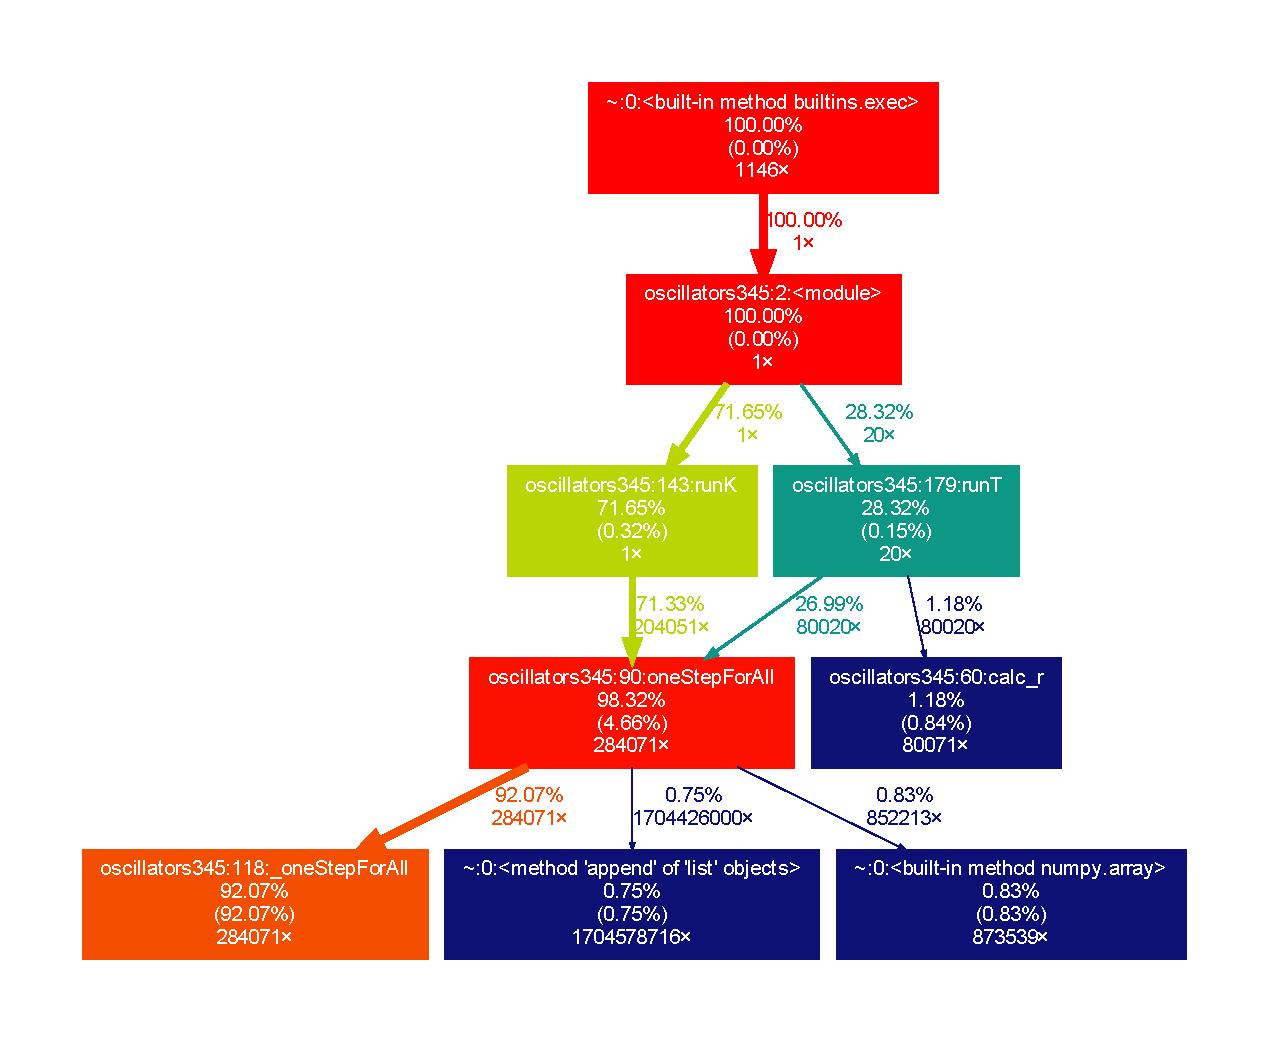
\includegraphics[width=\textwidth]{graphics/profile345.pdf} % can also use angle = 90
	\caption{Profile of code for task 3, 4 and 5}
	\label{profile345}
\end{figure}
%\end{landscape}


\subsubsection{Results}

\begin{figure}[h]
	\centering
	\begin{subfigure}{0.9\textwidth}
		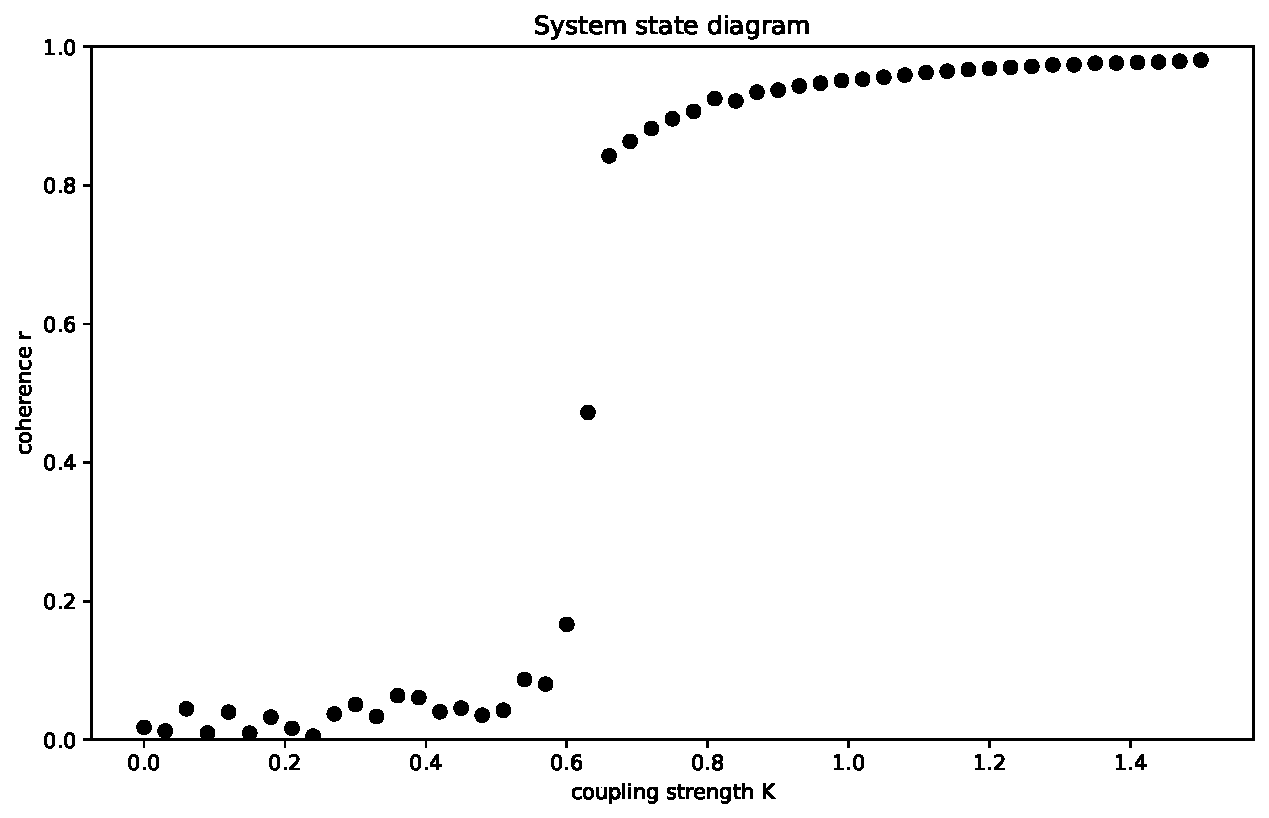
\includegraphics[width = \textwidth]{graphics/3_K-vs-r_omegaDistr=uniform_zoomed_N=2000_1611568972.pdf}
		\caption{zoomed in}
		\label{3zoomedin}
	\end{subfigure}
	\begin{subfigure}{0.9\textwidth}
		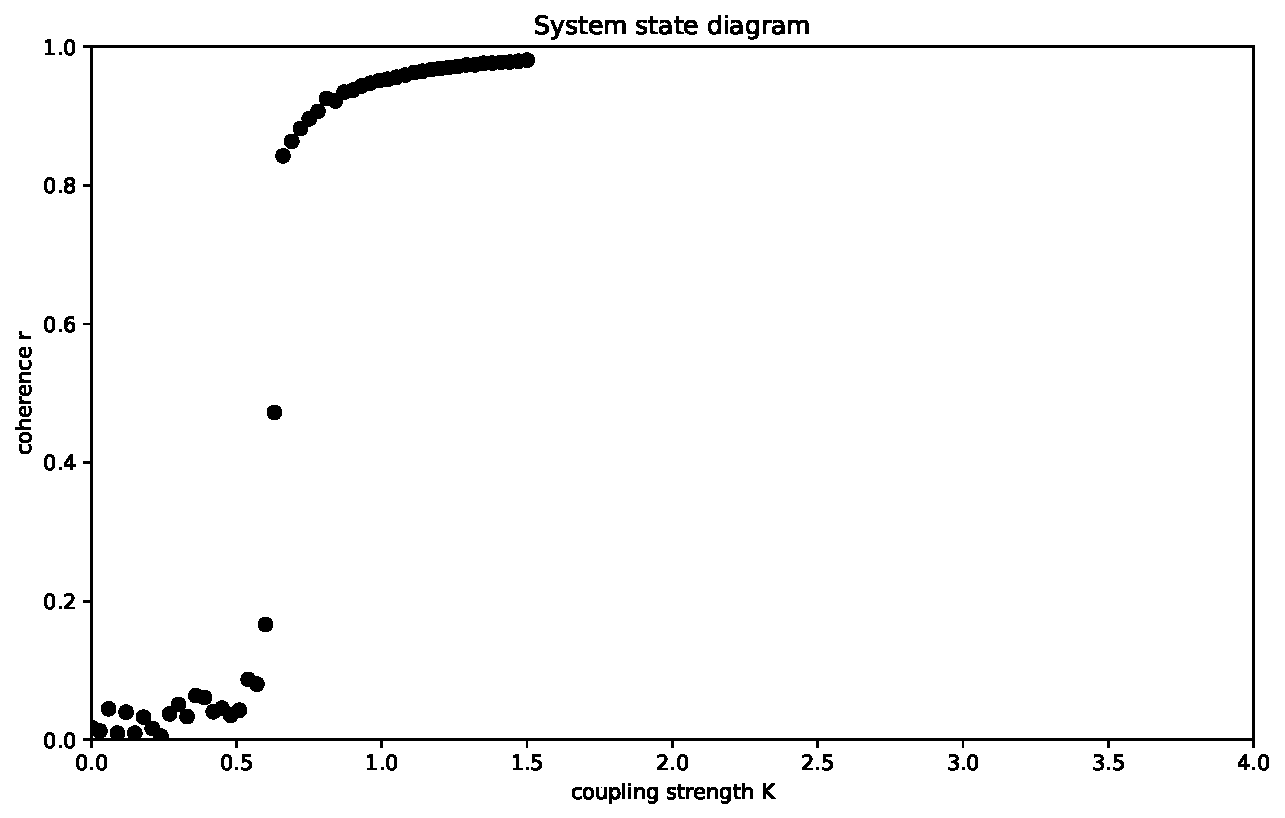
\includegraphics[width = \textwidth]{graphics/3_K-vs-r_omegaDistr=uniform_N=2000_1611568972.pdf}
		\label{3zoomedout}
		\caption{zoomed out, for better comparison with figure \ref{1}}
	\end{subfigure}
	\caption{$r_\infty(K)$ for different values of K, with a uniform distribution of $\omega$s}
	\label{3}
\end{figure}













%%%%%%%%%%%%%%%%%%%%%%%%%%%%%%%%%%%%%%%%%%%%%%%%%%%%%%%%%%%%%%%%%%%%%%%%%%%%%%%%%%%%%%%%%%%%%%%%%%%%%%%%%%%%%%%%%%%%%%%%%%%%%%%%%
\clearpage
\subsection{$r(t)$ for different initial conditions $\theta_0$}

To run simulations repeatedly while keeping selected initial conditions the same, I implemented the following. 
First, a 'reference' \oscpop object is initiated. 
Then a loop begins in which a 'temporary' \oscpop objects (newly initialised with entirely random values) is created. 
The desired initial conditions from the reference object are then written into the temporary object: here, the $\omega$s are kept, later the $\theta$s. 
\code{runT()} is executed on the temporary object and the returned trajectory saved into another list-of-lists. 








\subsubsection{Results}

\begin{figure}[h]
	\centering
	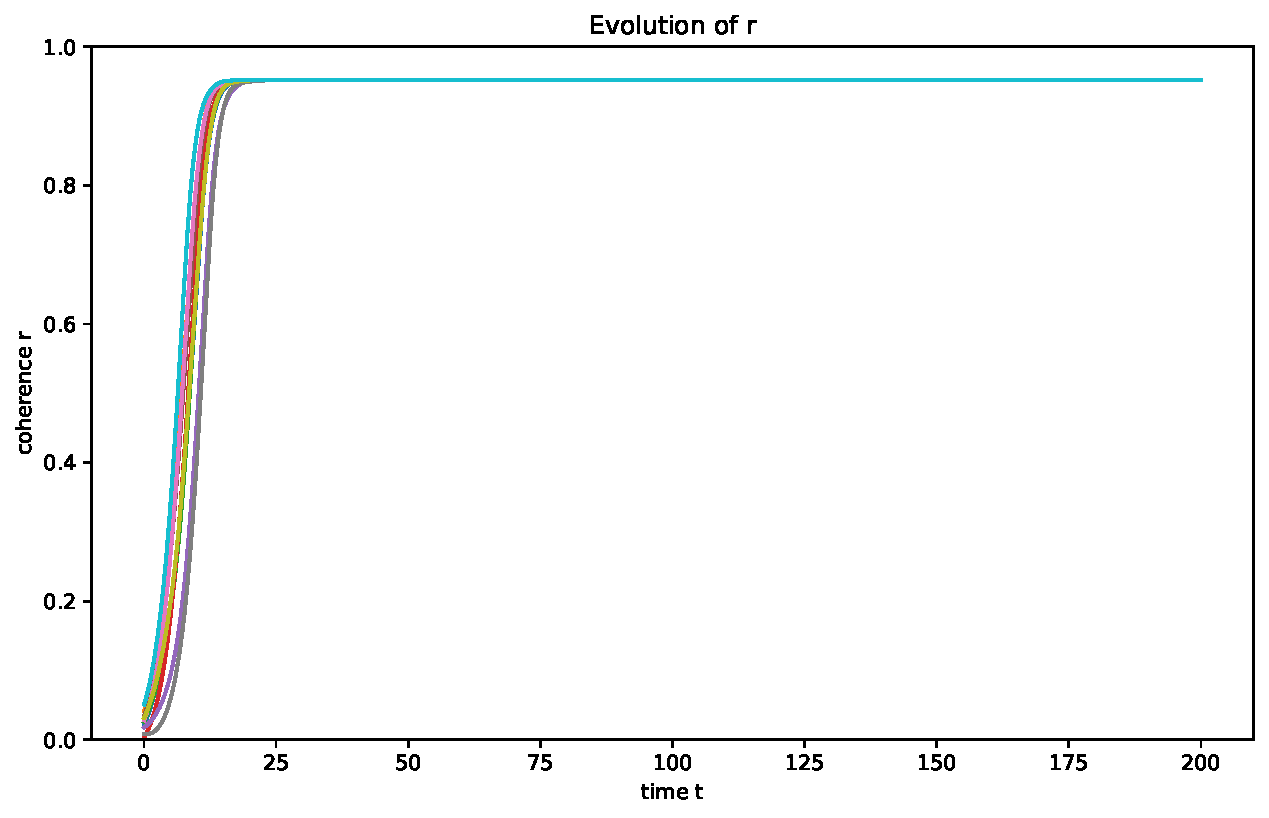
\includegraphics[width=0.9\textwidth]{graphics/4_t-vs-r_fixedOmegas_omegaDistr=uniform_N=2000_1611570486.pdf}
	\caption{$r(t)$ over time for 10 different initial conditions of $\theta$}
	\label{4}
\end{figure}











%%%%%%%%%%%%%%%%%%%%%%%%%%%%%%%%%%%%%%%%%%%%%%%%%%%%%%%%%%%%%%%%%%%%%%%%%%%%%%%%%%%%%%%%%%%%%%%%%%%%%%%%%%%%%%%%%%%%%%%%%%%%%%%%%
\clearpage
\subsection{$r(t)$ for different initial conditions $\omega_0$}






\subsubsection{Results}

\begin{figure}[h]
	\centering
	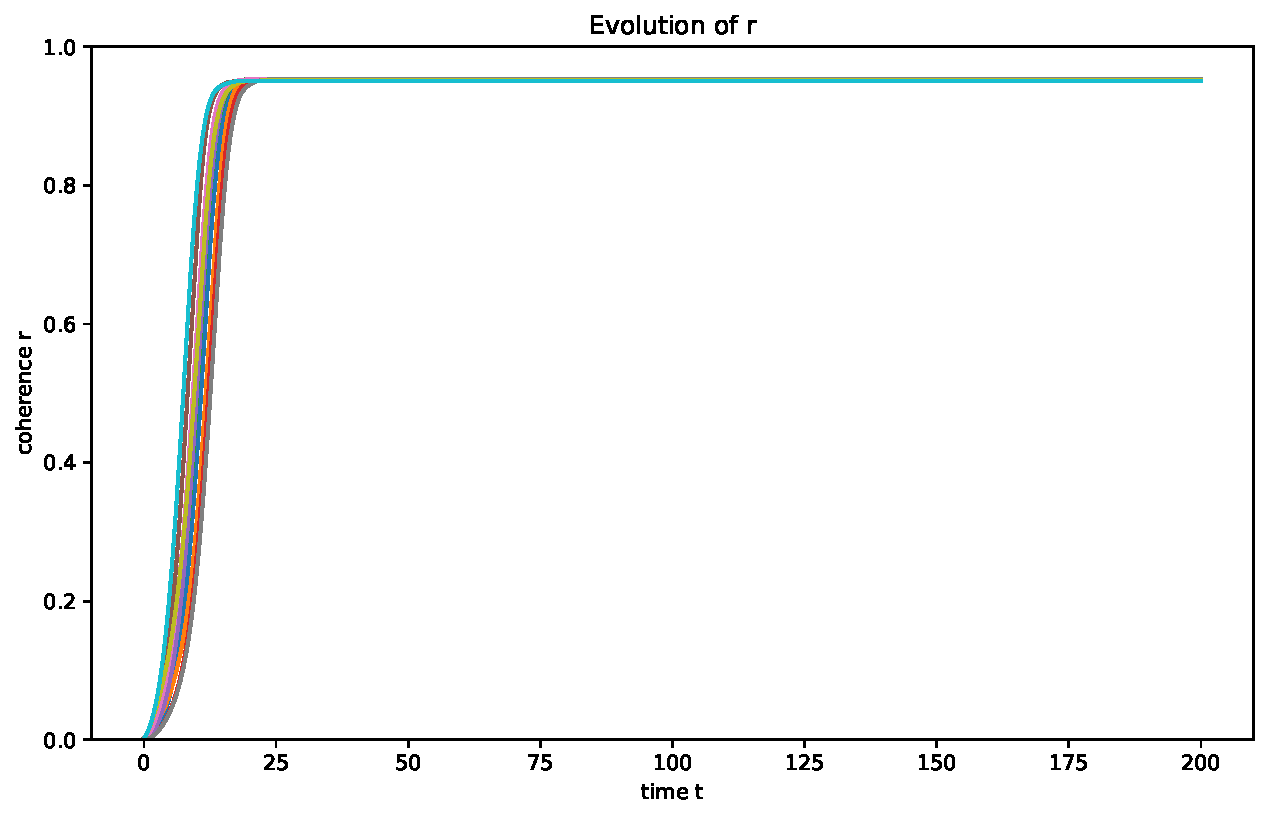
\includegraphics[width=0.9\textwidth]{graphics/5_t-vs-r_fixedThetas_omegaDistr=uniform_N=2000_1611572031.pdf}
	\caption{$r(t)$ over time for 10 different initial conditions of $\omega$}
	\label{5}
\end{figure}































\end{document}